\documentclass[24pt, a2papper, portrait]{tikzposter}
\usepackage[utf8]{inputenc}
\usepackage{blindtext}
\usepackage{comment}
 
\title{Who to follow on Twitter}
\author{Group 7: POSTER 1}
\date{\today}
\usetheme{Simple}

\begin{document}
\maketitle

\begin{columns}

    \column{0.5}
    \block{Problem description}{
        The objective of this paper is to implement a web application of a Twitter user
        recommender system. The application should, given a topic, recommend Twitter
        users to follow. The resulting engine uses tf-idf in combination with PageRank
        to recommend users. 
        \\\large{\textbf{Conclusion}} \\
        The conclusion is that it is feasible to create a Twitter
        user recommender engine using tf-idf and PageRank. Twitter data is suitable to
        be represented as a graph. Looking at the results, using appropriate parameters
        for weighing tf-idf and PageRank yields a result that is satisfying. Measuring
        the extent of the satisfaction is subjective, but for the group of this project
        it is deemed that the result is satisfactory enough for the given task.
    }

    \column{0.5}
    \block{The database} {
        \begin{tikzfigure}
            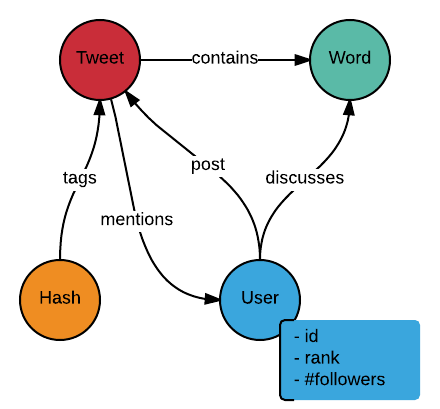
\includegraphics[width=.6\linewidth]{images/Schema.png}
        \end{tikzfigure}
        \begin{itemize}
          \item Number of users: 160.562
          \item Number of tweets: 1.021.876
          \item Number of words: 54.576
          \item Number of edges: 13.009.796
        \end{itemize}
    }

\end{columns}

\begin{columns}

    \column{0.5}
    \block{PageRank}{
        Nodes are users. Edges are mentions. User mentions are the links between
        the users (documents).

        \begin{tikzfigure}
            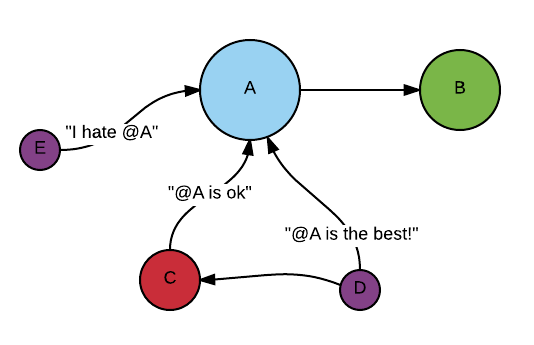
\includegraphics[width=.7\linewidth]{images/PageRank.png}
        \end{tikzfigure}
    }
    \column{0.5}
    \block{tf-idf}{
        tf: The term frequency is the number of times a term appears in a users
        tweets. \\
        df: The document frequency is the number of users that have talked about
        the term. \\

        tf-idf: The \emph{cosine-similarity} is used to compute how close the
        query is to each of the documents. \\

        A link between a \emph{User} node and a \emph{Word} node maps directly
        to a tf-idf score.
    }
\end{columns}

\begin{columns}
    \column{0.5}
    \block{Final Score}{
        After retrieving the sets of \emph{PageRank} and \emph{tf-idf} scores for all
        users that discuss any query term, they are normalized to zero-average and
        unitary variance so that they can be mixed together by means of a parameter,
        $\alpha$.  Finally both terms are combined, and the resulting score can be seen
        in Equation, where $s_t$ is the tf-idf score for user $u$
        and query $q$ and $s_p$ the PageRank score of $u$.

        \begin{equation}
            s(u,q) = \alpha * s_t(u,q) + (1 - \alpha) * s_p(u)
            \label{eq:finalscore}
        \end{equation}
    }

    \column{0.5}
    \block{Word2vec - Generating Synonyms} {
        For example: 
        \\"president" $\Rightarrow$ \textit{presidency, presidents, chairmen, presidential, governor, chairman}
        \\"liberal" $\Rightarrow$ \textit{conservative, liberals, liberalism, political, populist, moderate}

    }
\end{columns}

\end{document}
